%Include simulation results: both wave forms in time domain, and in frequency domain (apply FFT) (assignments 3 and 4 only).

Figure~\ref{fig:simulation:waveform} shows a comparison of the waveform for the input and the output audio.
As is shown here, these images are very similar.
This gives us a first indication that the output is indeed a resampled version of the input.
As shown on the left, the input has a sample rate of 44100Hz, while the output has a sample rate of 48000Hz.

\begin{figure}[H]
	\centering
	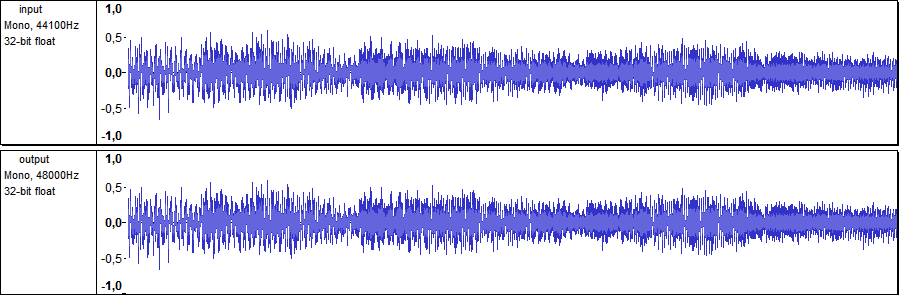
\includegraphics[width=0.9\textwidth]{comparison}
	\caption{Comparison of the waveform for the input and the output}
	\label{fig:simulation:waveform}
\end{figure}

If we zoom in a bit further, as can be seen in Figure~\ref{fig:simulation:waveformzoom}, the waveform of the input and the waveform of the output are still very similar.

\begin{figure}[H]
	\centering
	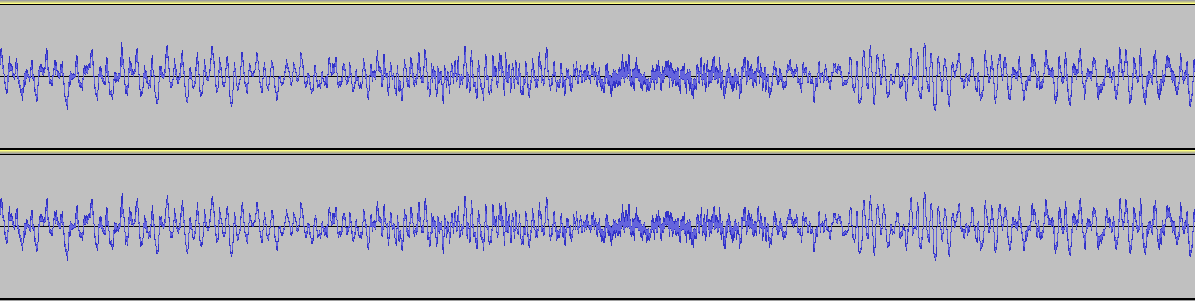
\includegraphics[width=0.9\textwidth]{comparison-zoom}
	\caption{Comparison of the waveform for the input and the output, zoomed in slightly}
	\label{fig:simulation:waveformzoom}
\end{figure}

Figure~\ref{fig:simulation:spectrum} shows the spectrum analysis of the input and the output files.
We can see that up to about 18kHz, the frequency analysis looks very much alike.
After that point, the input and output start to differ.
However, the instructor has assured us that this difference is negligible.

\begin{figure}[H]
	\centering
	\begin{subfigure}[l]{0.7\textwidth}
		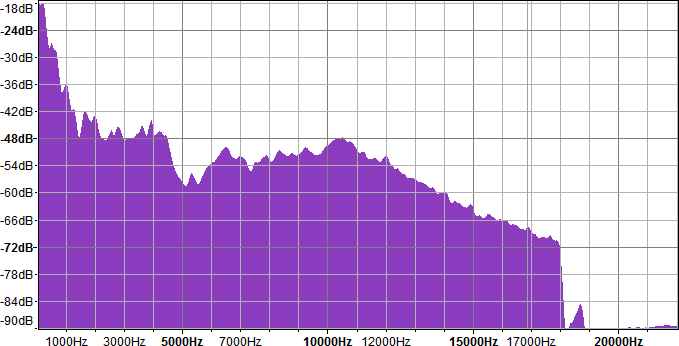
\includegraphics[width=\textwidth]{freq-input}
		\caption{Input}
		\label{fig:simulation:spectrum:before}
	\end{subfigure}

	\begin{subfigure}[l]{0.7\textwidth}
		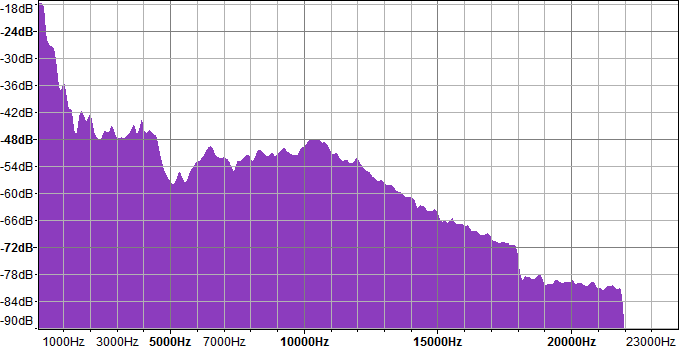
\includegraphics[width=\textwidth]{freq-output}
		\caption{Output}
		\label{fig:simulation:spectrum:after}
	\end{subfigure}

	\caption{Comparison of the audio spectrum before and after running the filter}
	\label{fig:simulation:spectrum}
\end{figure}

In Figure~\ref{fig:simulation:samples} we zoom in on the waveform even further.
This allows us to see individual samples.
We can see here that the output does indeed have a higher sample rate than the input.
Even on this level, the waveform of the input and the output are almost identical.
We have noticed, however, that there is a delay of around 4 output-samples (around 83 microseconds at 48000kHz) in the output, relative to the input.
While we can explain the first 4 output-samples being zero (the first two are due to the fact that we need more input to calculate an output, the third and the fourth are due to the fact that the first two coefficients are 0), we are not sure why this delay happens everywhere in the output.

However, since our design was allowed to have some start-up noise, we do not attempt to fix this.

\begin{figure}[H]
	\centering
	\begin{subfigure}[l]{\textwidth}
		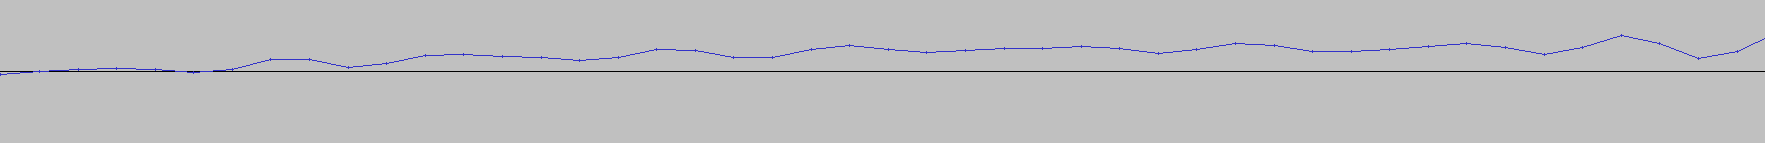
\includegraphics[width=\textwidth]{samples-input}
		\caption{Input}
		\label{fig:simulation:samples:before}
	\end{subfigure}

	\begin{subfigure}[l]{\textwidth}
		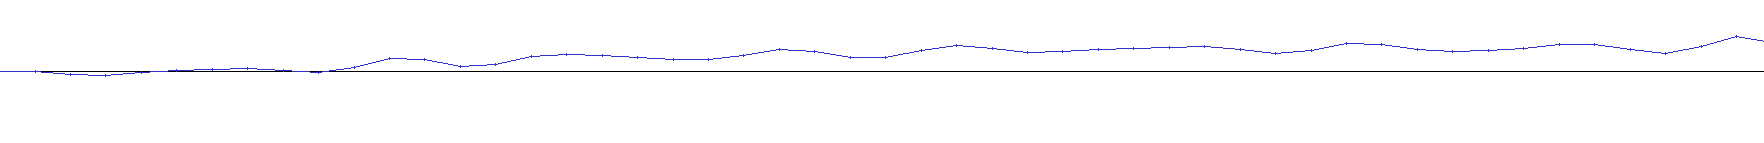
\includegraphics[width=\textwidth]{samples-output}
		\caption{Output}
		\label{fig:simulation:samples:after}
	\end{subfigure}

	\caption{Comparison of the waveform for the input and the output, zoomed from 5,890s to 5,891s}
	\label{fig:simulation:samples}
\end{figure}
